\documentclass[aspectratio=169]{beamer}
\usepackage{beamerthemesplit}
\usepackage{multirow}
\usepackage{array}
\usepackage{hyperref}
\usepackage[T1]{fontenc}
\usepackage{inconsolata}
\usepackage{xcolor,colortbl}
\usepackage{natbib}
\usepackage{listings}
\usepackage{physics}
\usepackage{centernot}
%%\newcommand{\newblock}{}
\DeclareGraphicsExtensions{.pdf,.png,.jpg}

%%\usetheme[pageofpages=of,% String used between the current page and the
%%                         % total page count.
%%          bullet=circle,% Use circles instead of squares for bullets.
%%          titleline=true,% Show a line below the frame title.
%%          alternativetitlepage=true,% Use the fancy title page.
%%          ]{Torino}
\usetheme{metropolis}
\definecolor{light-green}{RGB}{144,238,144}
\makeatletter
%%\setbeamertemplate{footline}
%%{
%%  \leavevmode%
%%  \hbox{%
%%  \begin{beamercolorbox}[wd=.333333\paperwidth,ht=2.25ex,dp=1ex,center]{author in head/foot}%
%%    \usebeamerfont{author in head/foot}\insertshortauthor~~\beamer@ifempty{\insertshortinstitute}{}{(\insertshortinstitute)}
%%  \end{beamercolorbox}%
%%  \begin{beamercolorbox}[wd=.333333\paperwidth,ht=2.25ex,dp=1ex,center]{title in head/foot}%
%%    \usebeamerfont{title in head/foot}\insertshorttitle
%%  \end{beamercolorbox}%
%%  \begin{beamercolorbox}[wd=.333333\paperwidth,ht=2.25ex,dp=1ex,right]{date in head/foot}%
%%    \usebeamerfont{date in head/foot}\insertshortdate{}\hspace*{2em}
%%%    \insertframenumber{} / \inserttotalframenumber\hspace*{2ex} % DELETED
%%  \end{beamercolorbox}}%
%%  \vskip0pt%
%%}
\makeatother
\newcommand\Wider[2][3em]{%
\makebox[\linewidth][c]{%
  \begin{minipage}{\dimexpr\textwidth+#1\relax}
  \raggedright#2
  \end{minipage}%
  }%
}
\begin{document}
\author{{\bf Casey Stella}\\@casey\_stella}
\title{{\bf Data Cleansing and Data Understanding}}
\subtitle{{\bf Best Practices and Lessons from the Field}}
\date{2017} 

\frame{\titlepage} 


\frame{\frametitle{Hi, I'm Casey Stella!}
\begin{itemize}
\item I'm a Principal Software Engineer at Hortonworks, a Hadoop vendor, writing open source software
\item I work on Apache Metron (Incubating), constructing a platform to do advanced analytics and data science for cyber security at scale\pause
\item Prior to this, I was
  \begin{itemize}
  \item Doing data science consulting on the Hadoop ecosystem for Hortonworks
  \item Doing data mining on medical data at Explorys using the Hadoop ecosystem
  \item Doing signal processing on seismic data at Ion Geophysical
  \item A graduate student in the Math department at Texas A\&M in algorithmic complexity theory
  \end{itemize}
\end{itemize}
}

\frame{\frametitle{Garbage In $\implies$ Garbage Out}
\begin{exampleblock}{}
  {\Large ``80\% of the work in any data project is in cleaning the data.''}
  \vskip5mm
  \hspace*\fill{\small--- D.J. Patel in {\em Data Jujitsu} }
\end{exampleblock}
}

\frame{\frametitle{Data Cleansing $\implies$ Data Understanding}
There are two ways to understand your data
\begin{itemize}
\item Syntactic Understanding
\item Semantic Understanding
\end{itemize}
If you hope to get anything out of your data, you have to have a handle on both.
}

\frame{\frametitle{Syntactic Understanding: True Types}
A {\bf true type} is a label applied to data points $x_i$ such that $x_i$ are mutually comparable.
\begin{itemize}
\item Schemas type != true data type
\item A specific column can have many different types
\end{itemize}\pause
``735'' has a true type of {\bf integer} but could have a schema type of {\bf string} or {\bf double}
}

\frame{\frametitle{Syntactic Understanding: Density}
Data {\bf density} is an indication of how data is clumped together.\pause
\begin{itemize}
  \item For numerical data, distributions and statistical characteristics are informative.\pause
  \item For non-numeric data, counts and distinct counts of a canonical representation are extremely useful.\pause
  \item For {\bf ALL} data, an indication of how ``empty'' the data is.\pause
\end{itemize}
Canonical representations are representations which give you an idea at a glance of the data format\pause
\begin{itemize}
  \item Replacing digits with the character `d'
  \item Stripping whitespace
  \item Normalizing punctuation
\end{itemize}\pause

{\bf Data density is an assumption underlying any conclusions drawn from your data.}
}

\frame{\frametitle{Syntactic Understanding: Density over Time}
{\bf $\frac{\Delta Density}{\Delta t}$} is how data clumps change over time.\pause

This kind of analysis can show
\begin{itemize}
\item Problems in the data pipeline\pause
\item Whether the assumptions of your analysis are violated\pause
\end{itemize}

$\frac{\Delta Density}{\Delta t}$ $\implies$
\begin{itemize}
  \item Automation\pause
  \item Outlier Alerting
\end{itemize}
}

\frame{\frametitle{Story Time: A Summation over Time Saves Face}
The stage: An unnamed startup analyzing clinical effectiveness measurement for hospital.\pause
\begin{itemize}
\item Think of it as a rules engine that takes medical data and outputs how well doctors and departments are doing\pause
\item Insights aren't trusted if they're wrong.\pause
\item Correctness depend on good data
\end{itemize}
}

\frame{\frametitle{Semantic Understanding: ``Do what I mean, not what I say''}
Semantic understanding is understanding based on how the data is {\bf used} rather than how it is stored.\pause
\begin{itemize}
\item Finding equivalences based on semantic understanding are often context sensitive.\pause
\item May come from humans (e.g. domain experience and ontologies)\pause
\item May come from machine learning (e.g. analyzing usage patterns to find synonyms)\pause
\end{itemize}
Semantic understanding {\bf may} require data science. At the same time, data science {\bf will} require semantic understanding.
}

\frame{\frametitle{Story Time: Very Busy Bags of Mostly Water; Very Confused Boxes of Silicon}
The stage: An unnamed insurance company building models to predict disease\pause
\begin{itemize}
\item Doctors and Nurses are busy people\pause
\item Humans suffer from confirmation bias\pause
\item Machines can only interpret what they can see\pause
\item Together we can fill in the gaps
\end{itemize}
}



\section{SummarizerCLI}

\begin{frame}[plain]
\Wider[4em]{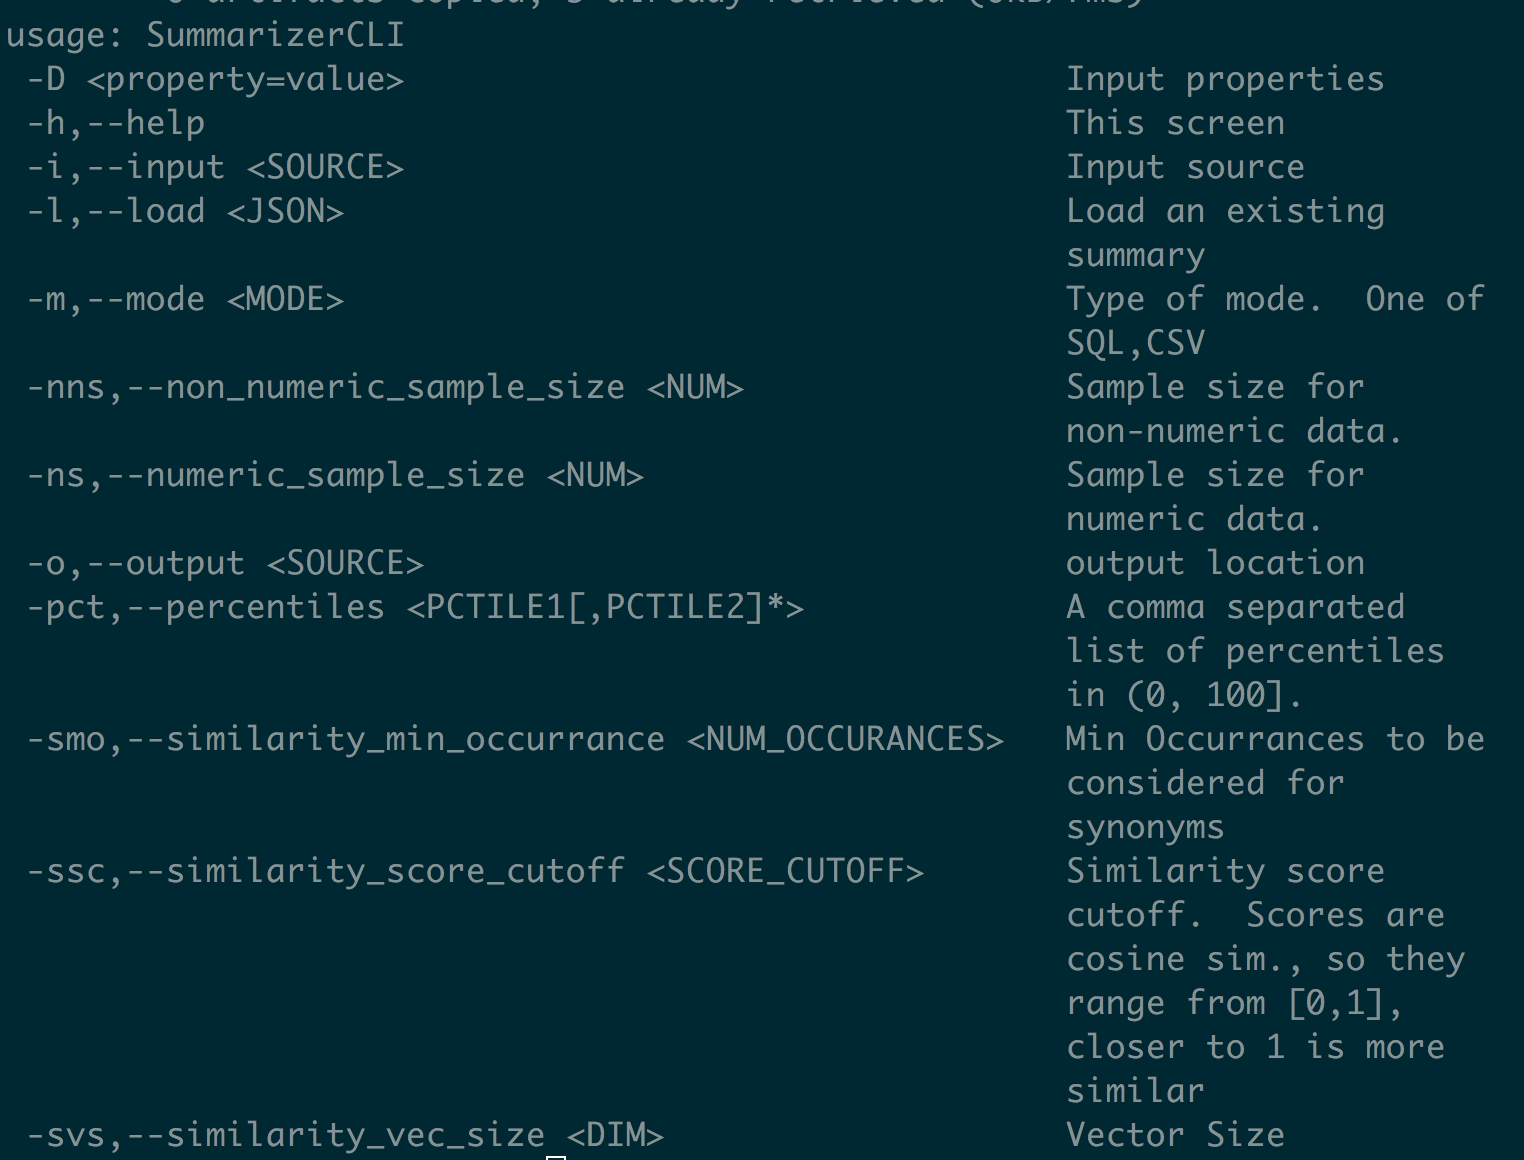
\includegraphics[scale=0.5]{0_usage.png}}
\end{frame}

\begin{frame}[plain]
\Wider[4em]{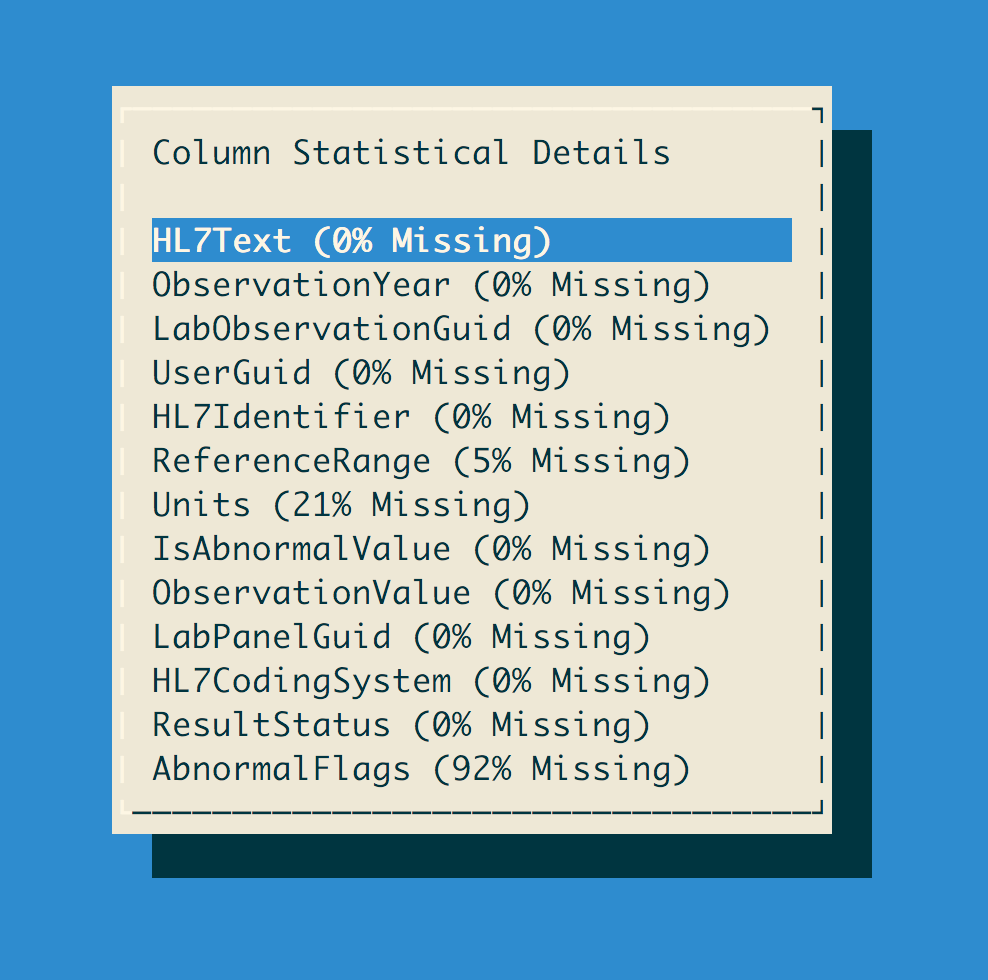
\includegraphics[scale=0.5]{1_column_list.png}}
\end{frame}

\begin{frame}[plain]
\Wider[4em]{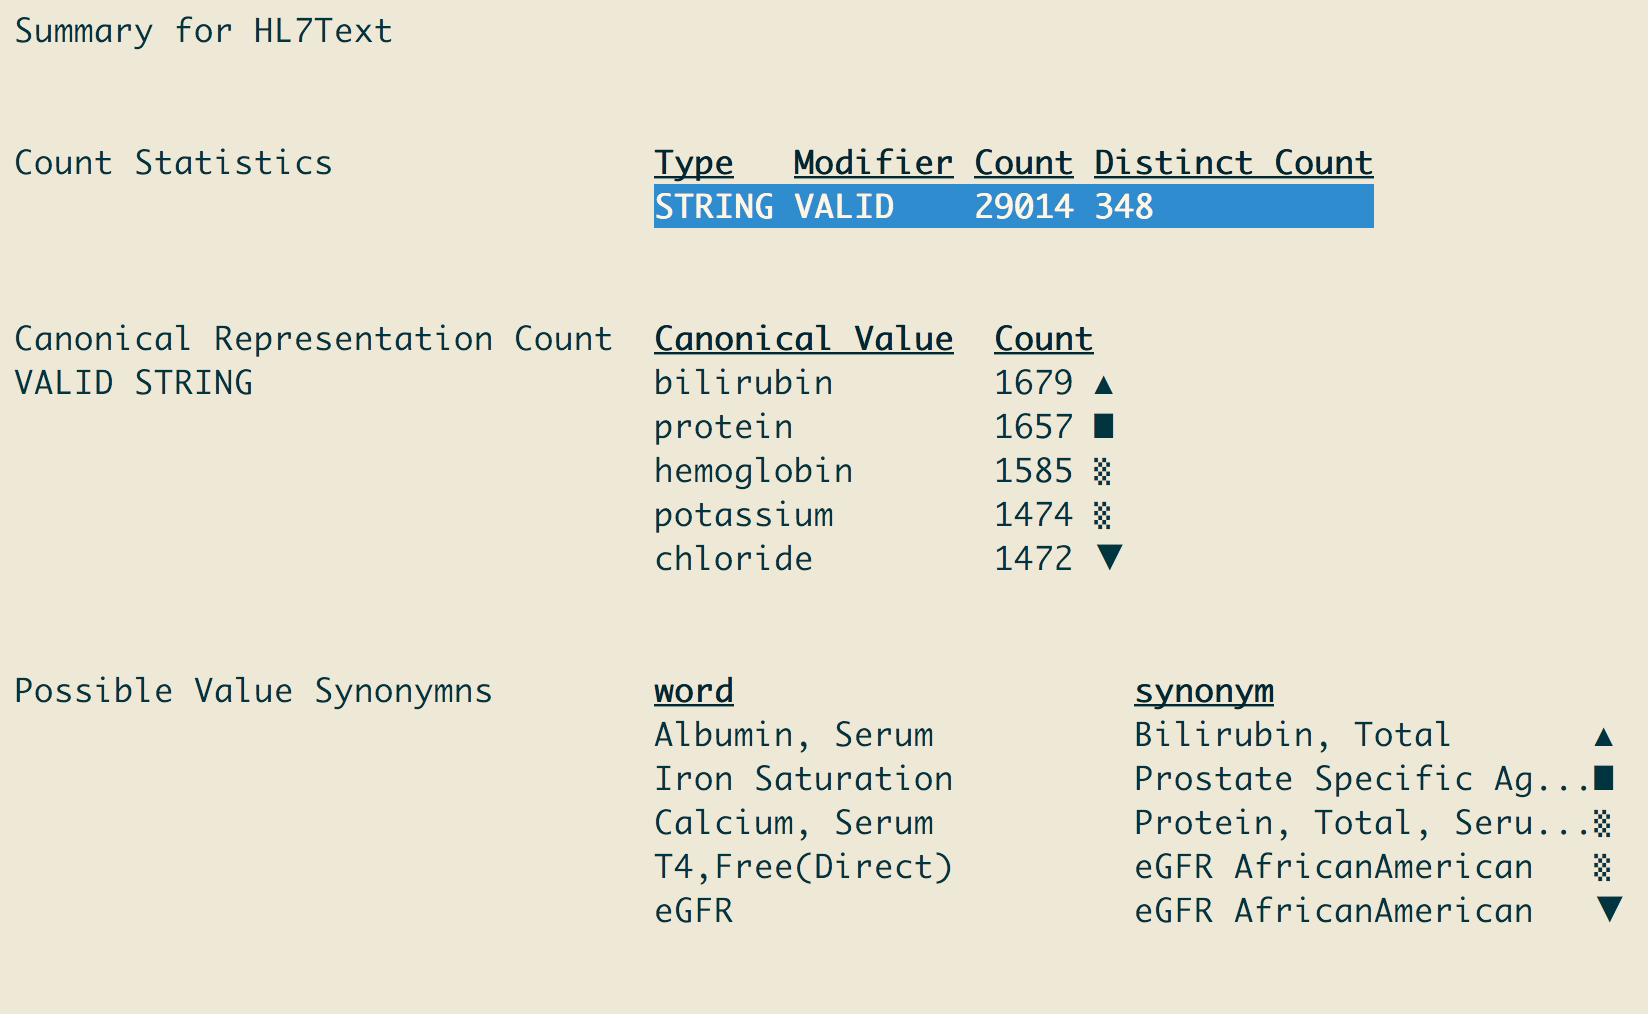
\includegraphics[scale=0.40]{2_hl7text.png}}
\end{frame}

\begin{frame}[plain]
\Wider[4em]{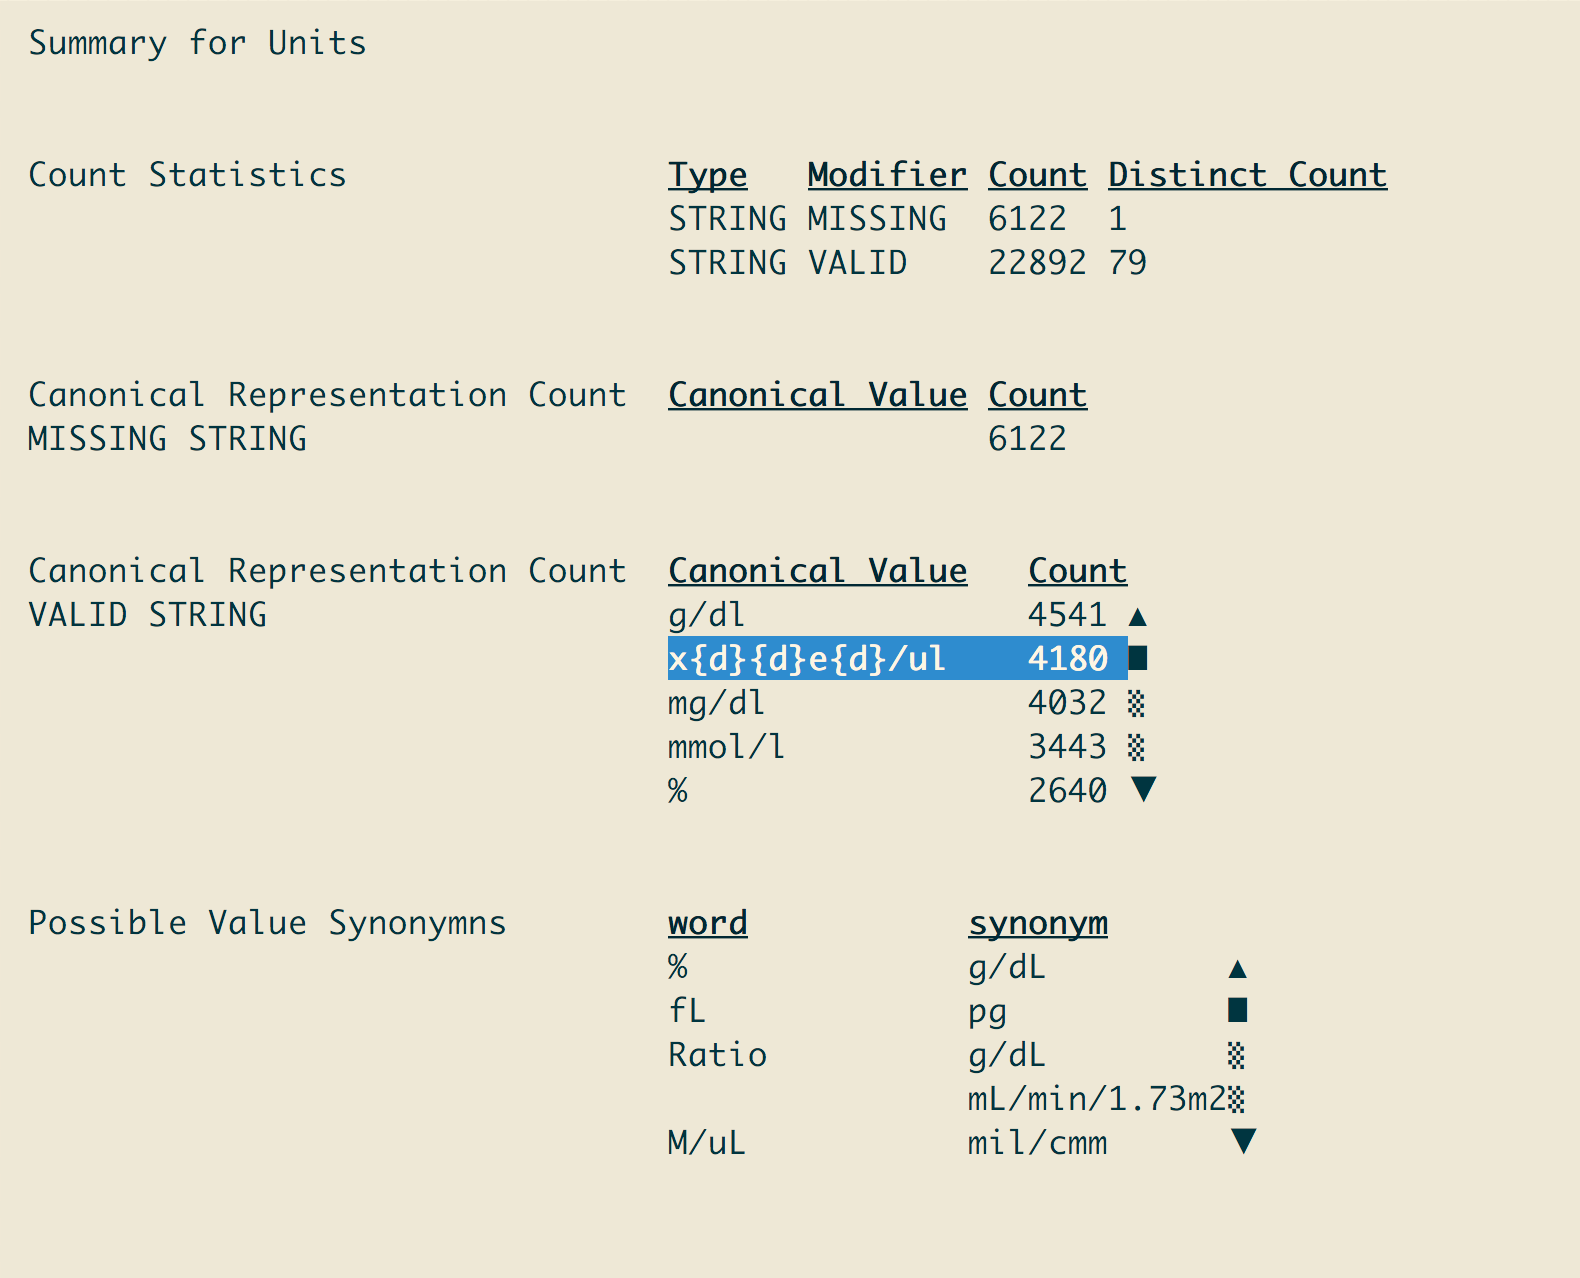
\includegraphics[scale=0.40]{3_units.png}}
\end{frame}

\frame{\frametitle{Implications for Team Structure}
To be successful,\pause
\begin{itemize}
\item Your data science teams have to be integrally involved in the data transformation and understanding.\pause
\item Your data science teams have to be {\bf willing} to get their hands dirty\pause
\item Your data science teams have to be {\bf allowed} to get their hands dirty\pause
\item Your data science teams need software engineering chops.
\end{itemize}
}



\section{Questions}

\frame{\frametitle{Questions}
Thanks for your attention!  Questions? 
\begin{itemize}
\item Code \& scripts for this talk available on my github presentation page.\footnote{http://github.com/cestella/presentations/}
\item Find me at http://caseystella.com 
\item Twitter handle: @casey\_stella 
\item Email address: cstella@hortonworks.com
\end{itemize}
}

\end{document}
